%%%%%%%%%%%%%%%%%%%%%%%%%%%%%%%%%%%%%%%%%
% Programming/Coding Assignment
% LaTeX Template
%
% This template has been downloaded from:
% http://www.latextemplates.com
%
% Original author:
% Ted Pavlic (http://www.tedpavlic.com)
%
% Note:
% The \lipsum[#] commands throughout this template generate dummy text
% to fill the template out. These commands should all be removed when 
% writing assignment content.
%
% This template uses a Perl script as an example snippet of code, most other
% languages are also usable. Configure them in the "CODE INCLUSION 
% CONFIGURATION" section.
%
%%%%%%%%%%%%%%%%%%%%%%%%%%%%%%%%%%%%%%%%%

%----------------------------------------------------------------------------------------
%	PACKAGES AND OTHER DOCUMENT CONFIGURATIONS
%----------------------------------------------------------------------------------------

\documentclass{article}

\usepackage{fancyhdr} % Required for custom headers
\usepackage{lastpage} % Required to determine the last page for the footer
\usepackage{extramarks} % Required for headers and footers
\usepackage[usenames,dvipsnames]{color} % Required for custom colors
\usepackage{graphicx} % Required to insert images
\usepackage{listings} % Required for insertion of code
\usepackage{courier} % Required for the courier font
\usepackage{lipsum} % Used for inserting dummy 'Lorem ipsum' text into the template

% Margins
\topmargin=-0.45in
\evensidemargin=0in
\oddsidemargin=0in
\textwidth=6.5in
\textheight=9.0in
\headsep=0.25in

\linespread{1.1} % Line spacing

% Set up the header and footer
\pagestyle{fancy}
\lhead{\hmwkAuthorName} % Top left header
\chead{\hmwkClass\ (\hmwkClassInstructor\ \hmwkClassTime): \hmwkTitle} % Top center head
\rhead{\firstxmark} % Top right header
\lfoot{\lastxmark} % Bottom left footer
\cfoot{} % Bottom center footer
\rfoot{Page\ \thepage\ of\ \protect\pageref{LastPage}} % Bottom right footer
\renewcommand\headrulewidth{0.4pt} % Size of the header rule
\renewcommand\footrulewidth{0.4pt} % Size of the footer rule

\setlength\parindent{0pt} % Removes all indentation from paragraphs

%----------------------------------------------------------------------------------------
%	CODE INCLUSION CONFIGURATION
%----------------------------------------------------------------------------------------

\definecolor{MyDarkGreen}{rgb}{0.0,0.4,0.0} % This is the color used for comments
\lstloadlanguages{Perl} % Load Perl syntax for listings, for a list of other languages supported see: ftp://ftp.tex.ac.uk/tex-archive/macros/latex/contrib/listings/listings.pdf
\lstset{language=Perl, % Use Perl in this example
        frame=single, % Single frame around code
        basicstyle=\small\ttfamily, % Use small true type font
        keywordstyle=[1]\color{Blue}\bf, % Perl functions bold and blue
        keywordstyle=[2]\color{Purple}, % Perl function arguments purple
        keywordstyle=[3]\color{Blue}\underbar, % Custom functions underlined and blue
        identifierstyle=, % Nothing special about identifiers                                         
        commentstyle=\usefont{T1}{pcr}{m}{sl}\color{MyDarkGreen}\small, % Comments small dark green courier font
        stringstyle=\color{Purple}, % Strings are purple
        showstringspaces=false, % Don't put marks in string spaces
        tabsize=5, % 5 spaces per tab
        %
        % Put standard Perl functions not included in the default language here
        morekeywords={rand},
        %
        % Put Perl function parameters here
        morekeywords=[2]{on, off, interp},
        %
        % Put user defined functions here
        morekeywords=[3]{test},
       	%
        morecomment=[l][\color{Blue}]{...}, % Line continuation (...) like blue comment
        numbers=left, % Line numbers on left
        firstnumber=1, % Line numbers start with line 1
        numberstyle=\tiny\color{Blue}, % Line numbers are blue and small
        stepnumber=5 % Line numbers go in steps of 5
}

% Creates a new command to include a perl script, the first parameter is the filename of the script (without .pl), the second parameter is the caption
\newcommand{\perlscript}[2]{
\begin{itemize}
\item[]\lstinputlisting[caption=#2,label=#1]{#1.pl}
\end{itemize}
}

%----------------------------------------------------------------------------------------
%	DOCUMENT STRUCTURE COMMANDS
%	Skip this unless you know what you're doing
%----------------------------------------------------------------------------------------

% Header and footer for when a page split occurs within a problem environment
\newcommand{\enterProblemHeader}[1]{
\nobreak\extramarks{#1}{#1 continued on next page\ldots}\nobreak
\nobreak\extramarks{#1 (continued)}{#1 continued on next page\ldots}\nobreak
}

% Header and footer for when a page split occurs between problem environments
\newcommand{\exitProblemHeader}[1]{
\nobreak\extramarks{#1 (continued)}{#1 continued on next page\ldots}\nobreak
\nobreak\extramarks{#1}{}\nobreak
}

\setcounter{secnumdepth}{0} % Removes default section numbers
\newcounter{homeworkProblemCounter} % Creates a counter to keep track of the number of problems

\newcommand{\homeworkProblemName}{}
\newenvironment{homeworkProblem}[1][Task \arabic{homeworkProblemCounter}]{ % Makes a new environment called homeworkProblem which takes 1 argument (custom name) but the default is "Problem #"
\stepcounter{homeworkProblemCounter} % Increase counter for number of problems
\renewcommand{\homeworkProblemName}{#1} % Assign \homeworkProblemName the name of the problem
\section{\homeworkProblemName} % Make a section in the document with the custom problem count
\enterProblemHeader{\homeworkProblemName} % Header and footer within the environment
}{
\exitProblemHeader{\homeworkProblemName} % Header and footer after the environment
}

\newcommand{\problemAnswer}[1]{ % Defines the problem answer command with the content as the only argument
\noindent\framebox[\columnwidth][c]{\begin{minipage}{0.98\columnwidth}#1\end{minipage}} % Makes the box around the problem answer and puts the content inside
}

\newcommand{\homeworkSectionName}{}
\newenvironment{homeworkSection}[1]{ % New environment for sections within homework problems, takes 1 argument - the name of the section
\renewcommand{\homeworkSectionName}{#1} % Assign \homeworkSectionName to the name of the section from the environment argument
\subsection{\homeworkSectionName} % Make a subsection with the custom name of the subsection
\enterProblemHeader{\homeworkProblemName\ [\homeworkSectionName]} % Header and footer within the environment
}{
\enterProblemHeader{\homeworkProblemName} % Header and footer after the environment
}

%----------------------------------------------------------------------------------------
%	NAME AND CLASS SECTION
%----------------------------------------------------------------------------------------

\newcommand{\hmwkTitle}{Assignment\ \#3} % Assignment title
\newcommand{\hmwkDueDate}{Tuesday,\ April\ 19,\ 2016} % Due date
\newcommand{\hmwkClass}{ILS - Z \ 604} % Course/class
\newcommand{\hmwkClassTime}{ } % Class/lecture time
\newcommand{\hmwkClassInstructor}{Prof. Xiazhong Liu} % Teacher/lecturer
\newcommand{\hmwkAuthorName}{vpatani (Vivek Patani)} % Your name

%----------------------------------------------------------------------------------------
%	TITLE PAGE
%----------------------------------------------------------------------------------------

\title{
\vspace{2in}
\textmd{\textbf{\hmwkClass:\ \hmwkTitle}}\\
\normalsize\vspace{0.1in}\small{Due\ on\ \hmwkDueDate}\\
\vspace{0.1in}\large{\textit{\hmwkClassInstructor\ \hmwkClassTime}}
\vspace{3in}
}

\author{\textbf{\hmwkAuthorName}}
\date{} % Insert date here if you want it to appear below your name

%----------------------------------------------------------------------------------------

\begin{document}

\maketitle

%----------------------------------------------------------------------------------------
%	TABLE OF CONTENTS
%----------------------------------------------------------------------------------------

%\setcounter{tocdepth}{1} % Uncomment this line if you don't want subsections listed in the ToC

\newpage
\tableofcontents
\newpage

%----------------------------------------------------------------------------------------
%	PROBLEM 1
%----------------------------------------------------------------------------------------

% To have just one problem per page, simply put a \clearpage after each problem

\begin{homeworkProblem}
Listing \ref{homework_example} Shows the IPynb Script.
\perlscript{homework_example}{Shows the IPynb Script for cleaning}

\begin{itemize}
\item How to configure the graphLab for AWS:

\begin{itemize}
\item Register as a student and Dato will send you a key.
\item Register the key as $graphlab.product-key$ function as shown above.
\item Execute in order to register
\end{itemize}

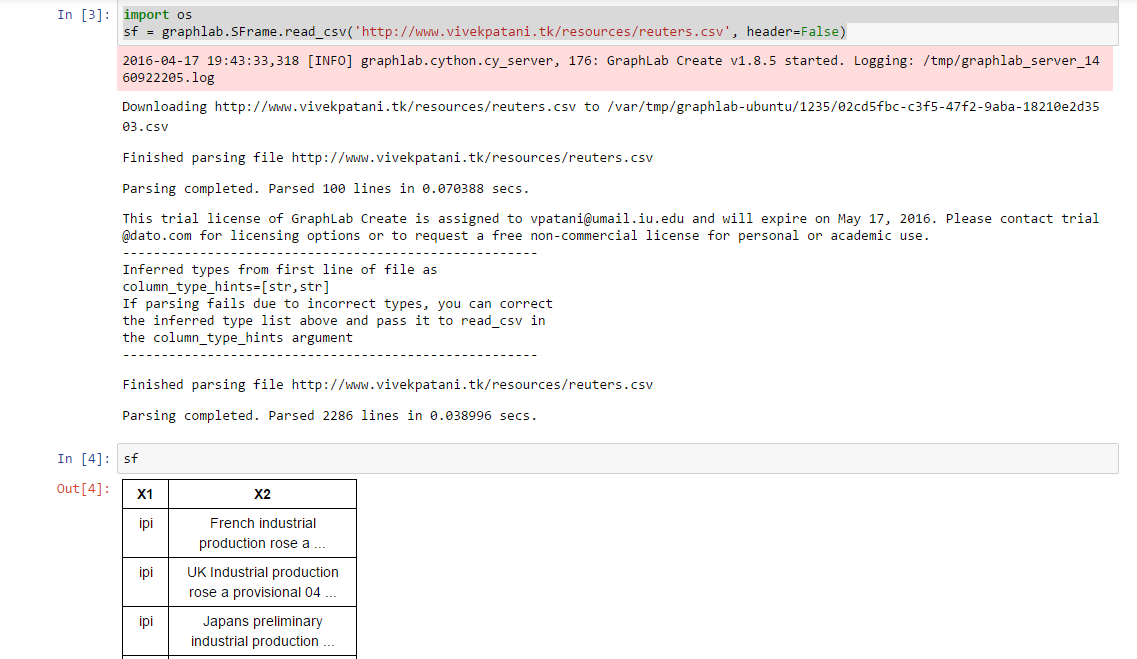
\includegraphics[width=0.75\columnwidth]{importing} % Importing

Listing \ref{homework_example2} Shows the IPynb Script.
\perlscript{homework_example2}{Shows the IPynb Script for counting}

\item Now we count the words and eliminate the stop words and words not crossing threshold

\begin{itemize}
\item Use the $SFrame.read - csv$ function giving input of the location of your file.
\item View sf to confirm the number of rows.
\item Once we have the data ready, we use the libraries to count the words that exist in the dataset. We use an Sarray.SArray to store the word and their count.
\item The next step is to see what words have appeared lesser than 2 times and we pass a parameter as 2 to the function $trim-by-value$.
\item Next step is to eliminate the stop word. We pass $doc$ as the input and the the output is over ridden on $doc$ itself by passing it through $stopwords$ function.
\item Just to make sure we've got it right, just check $doc[0]$.
\end{itemize}

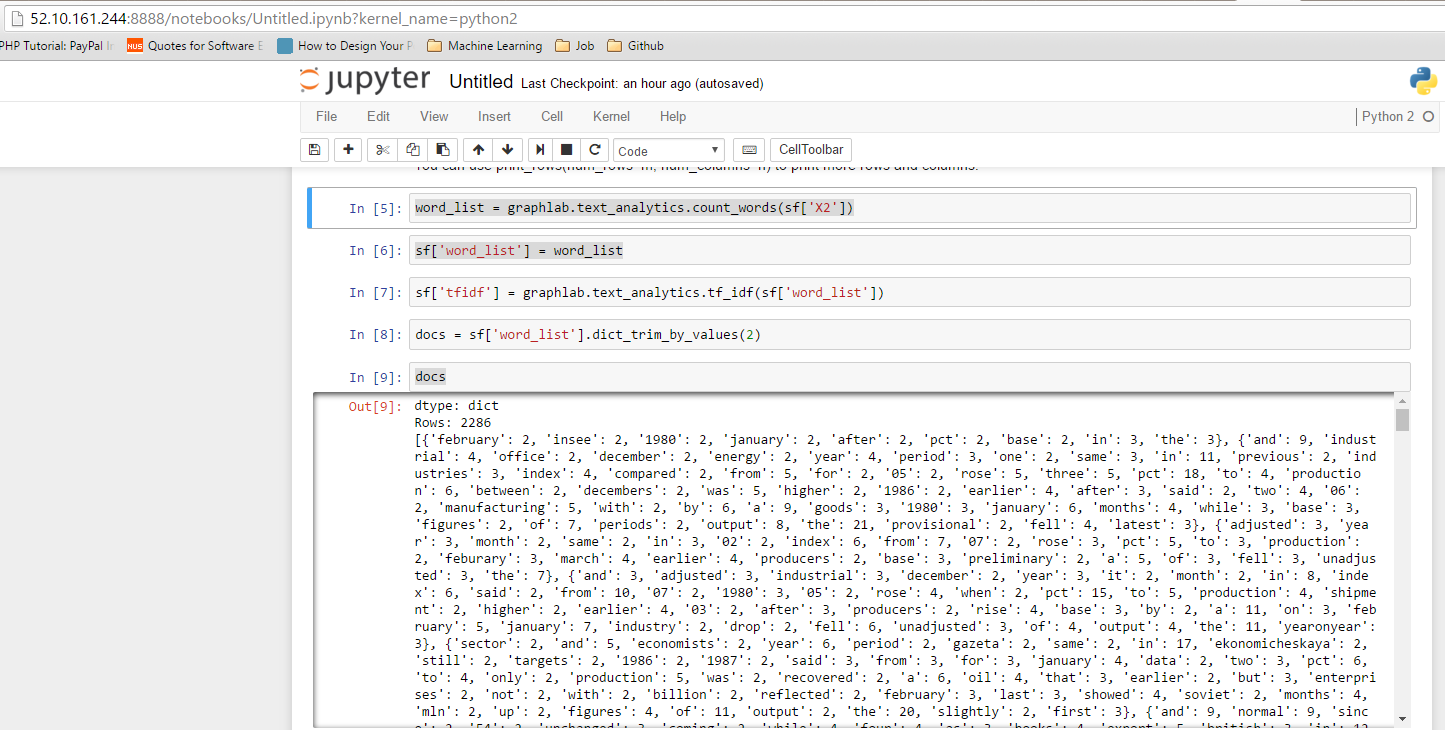
\includegraphics[width=0.75\columnwidth]{wordList}\\~\\ % Preprocessing.\\
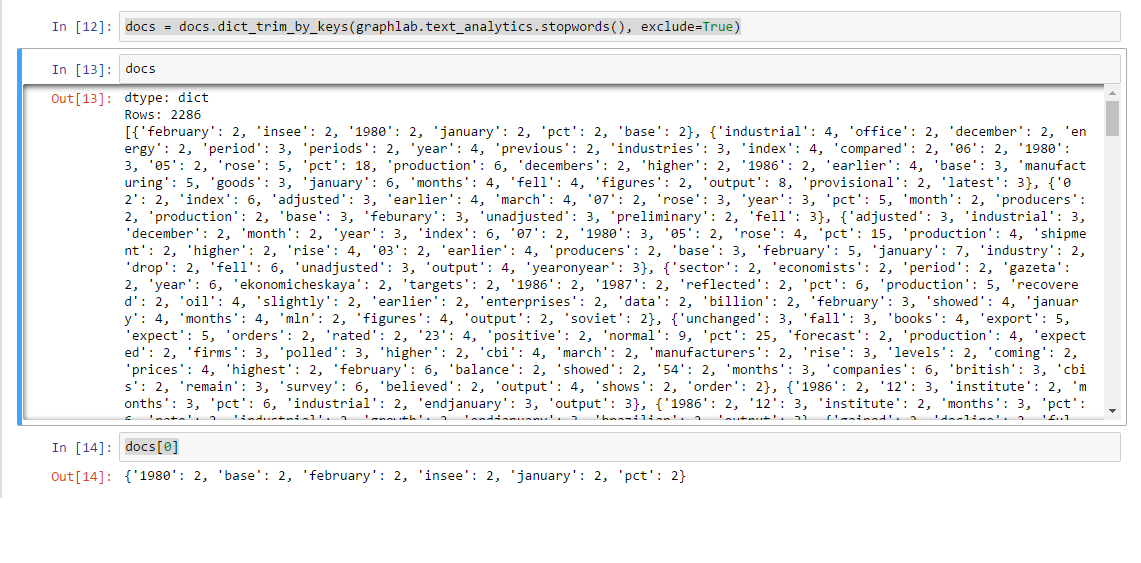
\includegraphics[width=0.75\columnwidth]{trimmed} % Preprocessing.

\item This completes the first part of \textbf{cleaning data} and \textbf{generating features}.

\end{itemize}

\end{homeworkProblem}


%----------------------------------------------------------------------------------------
%	PROBLEM 2
%----------------------------------------------------------------------------------------

\clearpage
\begin{homeworkProblem}

Listing \ref{homework_example3} Shows the IPynb Script.
\perlscript{homework_example3}{Shows the IPynb Script for generating Features}

\begin{itemize}
\item Here the we simply create a list(bag) of words for each document.
\item This is straightforward since we just generate a word list by the $count_words$ function by giving input as the the feature column over which we need to do this.
\item Next step is to add it the frame generated by us.
\item Next run the TF-IDF from the analytics library of graph lab over the word list generated.
\item We generated two things
\begin{enumerate}
\item Word List
\item TF-IDF Values
\end{enumerate}
\item This is how the Frame will look like\\
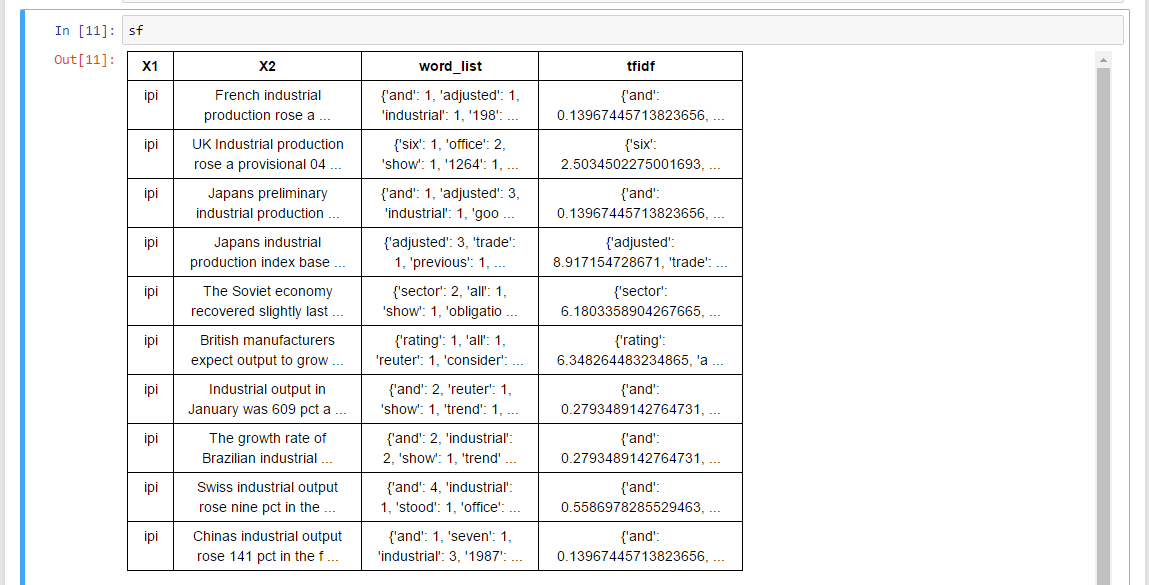
\includegraphics[width=0.75\columnwidth]{partthree} % Example image
\item Now, we have attached the \textbf{features} that will help us analyse the data.
\end{itemize}

\end{homeworkProblem}


%----------------------------------------------------------------------------------------


%----------------------------------------------------------------------------------------
%	PROBLEM 3
%----------------------------------------------------------------------------------------
\clearpage
\begin{homeworkProblem}
Listing \ref{homework_example4} Shows the IPynb Script.
\perlscript{homework_example4}{Shows the IPynb Script for generating Model \& Evaluating it}

\begin{itemize}

\item In this we have cleaned the data and build the elements required to build a model.
\item We first divide the set into \textbf{Train} \& \textbf{Test} in order to build and evaluate the model. We split the data in the ratio of 80:20, where 80 is train and 20 is test.
\item This is how the Train \& Test Frame will look like\\
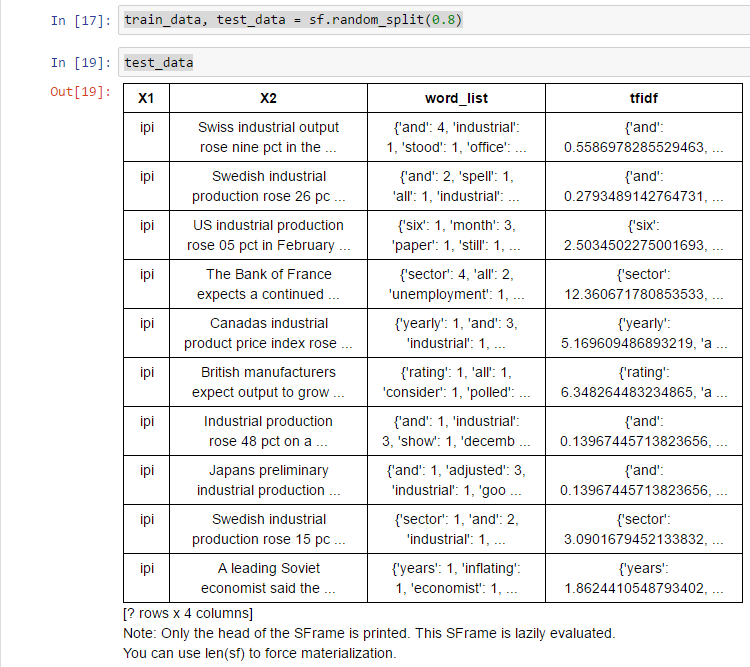
\includegraphics[width=0.75\columnwidth]{testtrain} % Example image

\item The length of each is\\
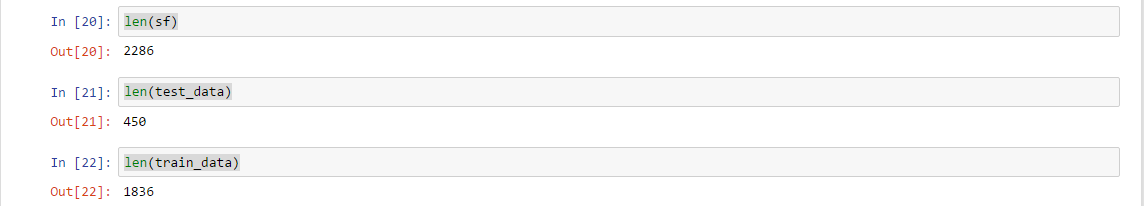
\includegraphics[width=0.75\columnwidth]{split} % Example image
\item We use train to learn the model and data.
\item Test will be used to evaluate features of the model such as accuracy.

\item Now we start building models with different approaches:
\begin{enumerate}


\item Boosted Tree Classifier:
Listing \ref{homework_example5} Shows the IPynb Script.
\perlscript{homework_example5}{Shows the IPynb Script for generating Model \& Evaluating it}
\begin{itemize}
\newpage
\item After training the data with the given model.
\item Output:\\
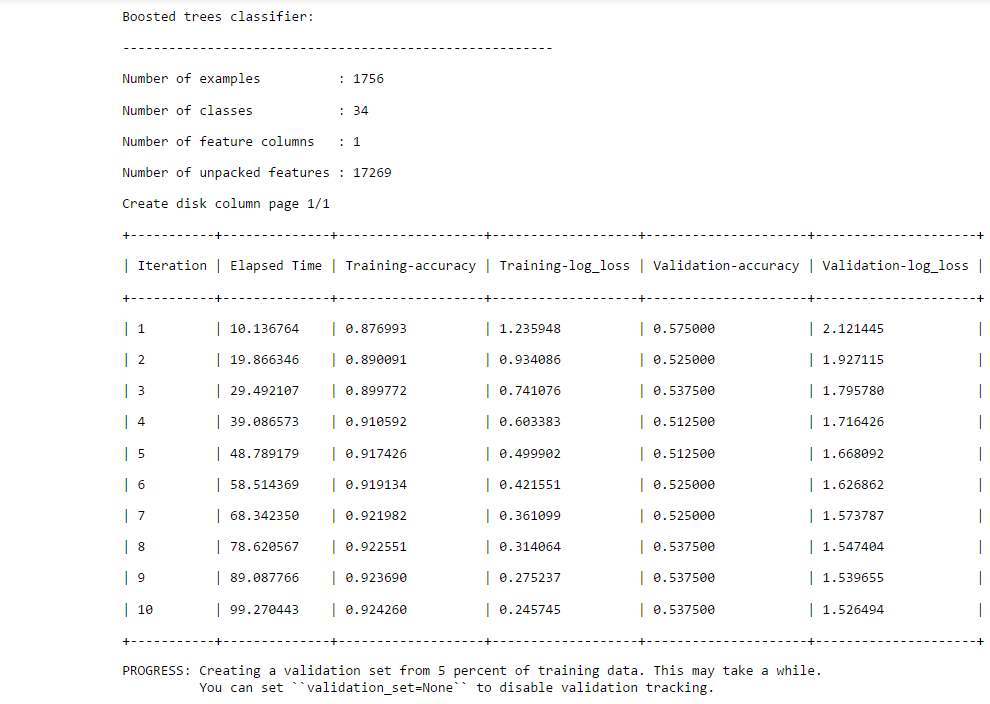
\includegraphics[width=0.75\columnwidth]{model1-1} % Example image

\newpage
\item After running the test, the accuracy is 71\%:
\item Output:\\
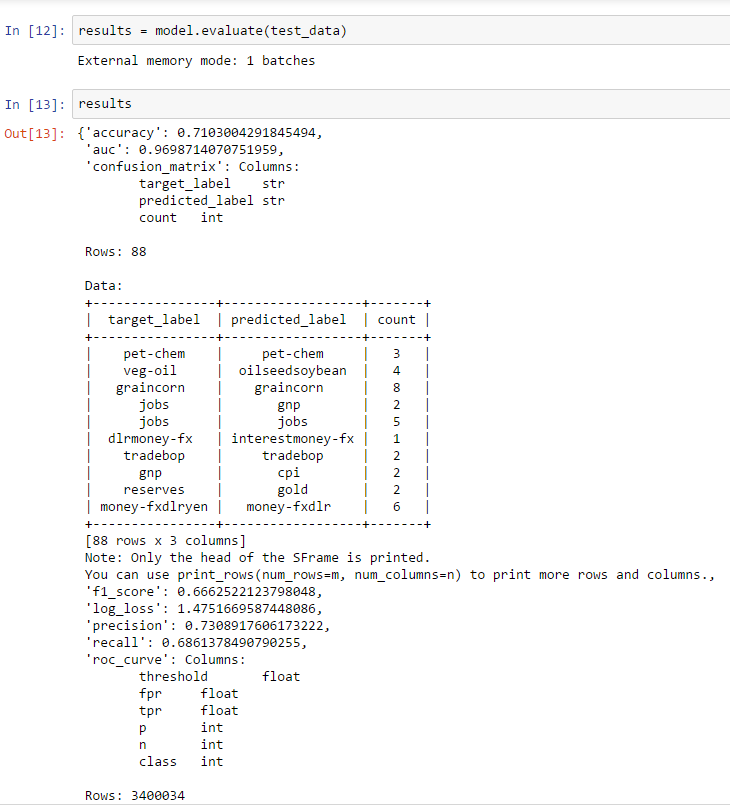
\includegraphics[width=0.75\columnwidth]{model1-2} % Example image

\newpage
\item The prediction excerpt
\item Output:\\
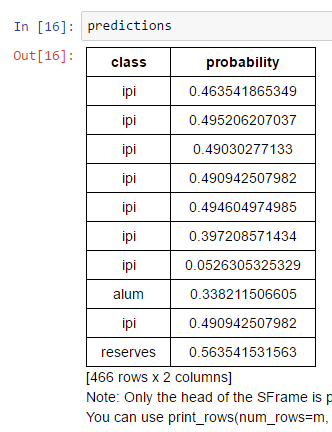
\includegraphics[width=0.75\columnwidth]{model1-3} % Example image

\end{itemize}


\item 
\end{enumerate}


\end{itemize}

\end{homeworkProblem}

%----------------------------------------------------------------------------------------

\end{document}